% !TeX root = ../main.tex

\chapter{绪论}

\section{编译器设计竞赛简介}

\subsection{发起背景}

编译原理一直以来都是计算机科学的重点研究方向和热门话题,为检验人才培养成效,计算机类教指委和系统能力培养专家组于2020年共同发起首届 “全国大学生计算机系统能力大赛编译系统设计赛(华为毕昇杯)”。该赛事面向全国高校本科生,以鼓励学生设计、实现一个综合性的编译系统,展示面向特定目标平台的编译器构造与编译优化的能力为目标,提升参赛者在计算机系统设计、分析、优化、应用方面的能力,是我国高校编译系统领域唯一的学科竞赛。

编译系统设计赛要求各参赛队综合运用各种知识(包括但不局限于编译技术、操作系统、计算机体系结构等),构思并实现一个综合性的编译系统,以展示面向特定目标平台的编译器构造与编译优化的能力。
本文就着重对这次比赛由来自中国科学技术大学的队伍“燃烧我的编译器”队的特等奖项目进行了分析和总结,挖掘和研究了项目中的亮点之处。

\subsection{竞赛评分标准}

大赛要求各参赛队综合运用前文提及的各种计算机系统能力知识,设计一个综合性的编译系统,各参赛队可自行决定编译器体系结构、前端与后端设计、代码优化等细节,同时需要兼顾编译器的迁移能力,纠错能力,拓展能力。因此,本次比赛对编译器的设计提出了较高要求,较为接近一个现代编译器的简化设计。

参赛队伍的项目需要通过各个基本的功能测试用例和性能基准测试用例,在通过功能测试的前提下,记录每个基准测试在目标硬件平台上的执行时间作为评价依据。

\subsection{编译器面向语言SysY简介}

SysY 语言是本次大赛要实现的编程语言,是 C 语言的一个子集。每个 SysY程序的源码存储在一个扩展名为sy的文件中。该文件中有且仅有一个名为main的主函数定义,还可以包含若干全局变量声明、常量声明和其他函数定义。SysY语言支持int类型和元素为int类型且按行优先存储的多维数组类型,其中int型整数为32位有符号数;const修饰符用于声明常量。

SysY 语言本身没有提供输入/输出(I/O)的语言构造,I/O是以运行时库方式提供,库函数可以在SysY程序中的函数内调用。

函数:函数可以带参数也可以不带参数,参数的类型可以是int或者数组类型;函数可以返回 int 类型的值,或者不返回值(即声明为 void 类型)。当参数为int时,按值传递;而参数为数组类型时,实际传递的是数组的起始地址,并且形参只有第一维的长度可以空缺。函数体由若干变量声明和语句组成。

变量/常量声明:可以在一个变量/常量声明语句中声明多个变量或常量,声明时可以带初始化表达式。所有变量/常量要求先定义再使用。在函数外声明的为全局变量/常量,在函数内声明的为局部变量/常量。

语句:语句包括赋值语句、表达式语句(表达式可以为空)、语句块、if 语句、while 语句、break语句、continue语句、return语句。语句块中可以包含若干变量声明和语句。

表达式:支持基本的算术运算、关系运算和逻辑运算,真假的表示和界定,关系或逻辑运算的结果,算符的优先级和和结合性以及计算规则(含逻辑运算的“短路计算”)均与 C 语言一致。

\section{论文和项目简要介绍}

\subsection{项目简介}

来自中国科学技术大学的队伍设计的项目“燃烧我的编译器”(下称,本项目)在本次比赛中取得了特等奖的\href{https://compiler.educg.net/2020CSDC}{最好成绩}。该项目已经在Github上开源,网址:\href{https://github.com/mlzeng/CSC2020-USTC-FlammingMyCompiler/}{https://github.com/mlzeng/CSC2020-USTC-FlammingMyCompiler/}。

项目设计上采用类LLVM的三段式编译器架构但别出新意,同时又有很多创新点,且易于阅读学习,开发时支持详细的自动化开发功能验证文件,并能生成详细的汇编代码注释。此外,本项目的拓展性较好,得益于使用了与机器或特定语言无关的中间表示形式IR来组织源代码解析的结果,可以方便的设计成C或其它语言的编译器,并利于迁移到其他常见架构平台。

最关键的是,本项目具有极强的优化能力,作为一个学习用的编译器,在针对SysY语言的大多数比赛测试用例时,在目标机树莓派4B上拥有超过GCC -O3的优化能力。除了简单编译器的经典优化如死代码消除,循环不变量外提,函数内联等优化,本项目还充分利用了树莓派ARM Cortex A7的4核处理器,设计并独创了创新多线程框架,可以更好的降低寄存器切换的开销,使得项目性能在决赛中脱颖而出。

\subsection{项目架构}

典型的三段式编译器架构如图~\ref{fig:arch}:
\\

\begin{figure}[htb]
  \centering
  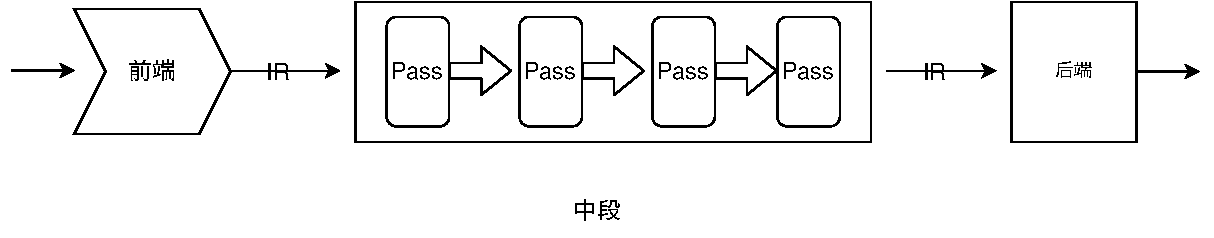
\includegraphics[width=0.9\textwidth]{figures/llvm.pdf}
  \caption{编译器的三段式设计}
  \label{fig:arch}
\end{figure}

而本项目对中端做了进一步的拓展,并细分了后端表示中虚拟指令的“底层程度”,下面对各个层次的架构进行简要说明。

首先,前端读取SysY源代码,使用Flex进行词法分析,生成token流,在这一步中,编译器主要是识别特殊符号,字符串,关键字和标识符等。然后进行语法分析,将token流的形式组织成抽象语法树AST。最后前端需要采用访问者模式遍历抽象语法树,生成与机器无关的中间表示,即生成IR,严格意义上的IR与特定的编程语言和机器架构实现都无关,这样便于拓展和移植编译器项目。

但是为降低从AST得到IR的难度,即尽量使得IR描述能力接近高级编程语言。同时,后端又希望IR可以方便的转化为机器码,即希望IR能够方便的翻译到底层汇编语言。为了联系这些看起来非常难同时实现的要求,计算机科学领域的其他实现已经告诉我们了答案:分层。本项目采用了三层IR的设计(High IR、Middle IR、Low IR),使用HIR弥补通用IR和AST的差距,使用LIR缩小IR和asm的差距。第二章中会简要介绍本项目的三层IR机制。

项目的后端负责IR到机器码的生成,结合ARM汇编的指令,负责寄存器分配和硬件资源的进一步利用,与中间代码优化的低层 IR Pass 相配合共同完成指令融合、调度和选择等优化。后端部分包含三个层次的虚拟指令,上层指令会选择最小代价智能翻译成一系列下层指令,在第四章会简要介绍。

整个编译过程可以描述为如下的流程。

\begin{figure}[htb]
  \centering
  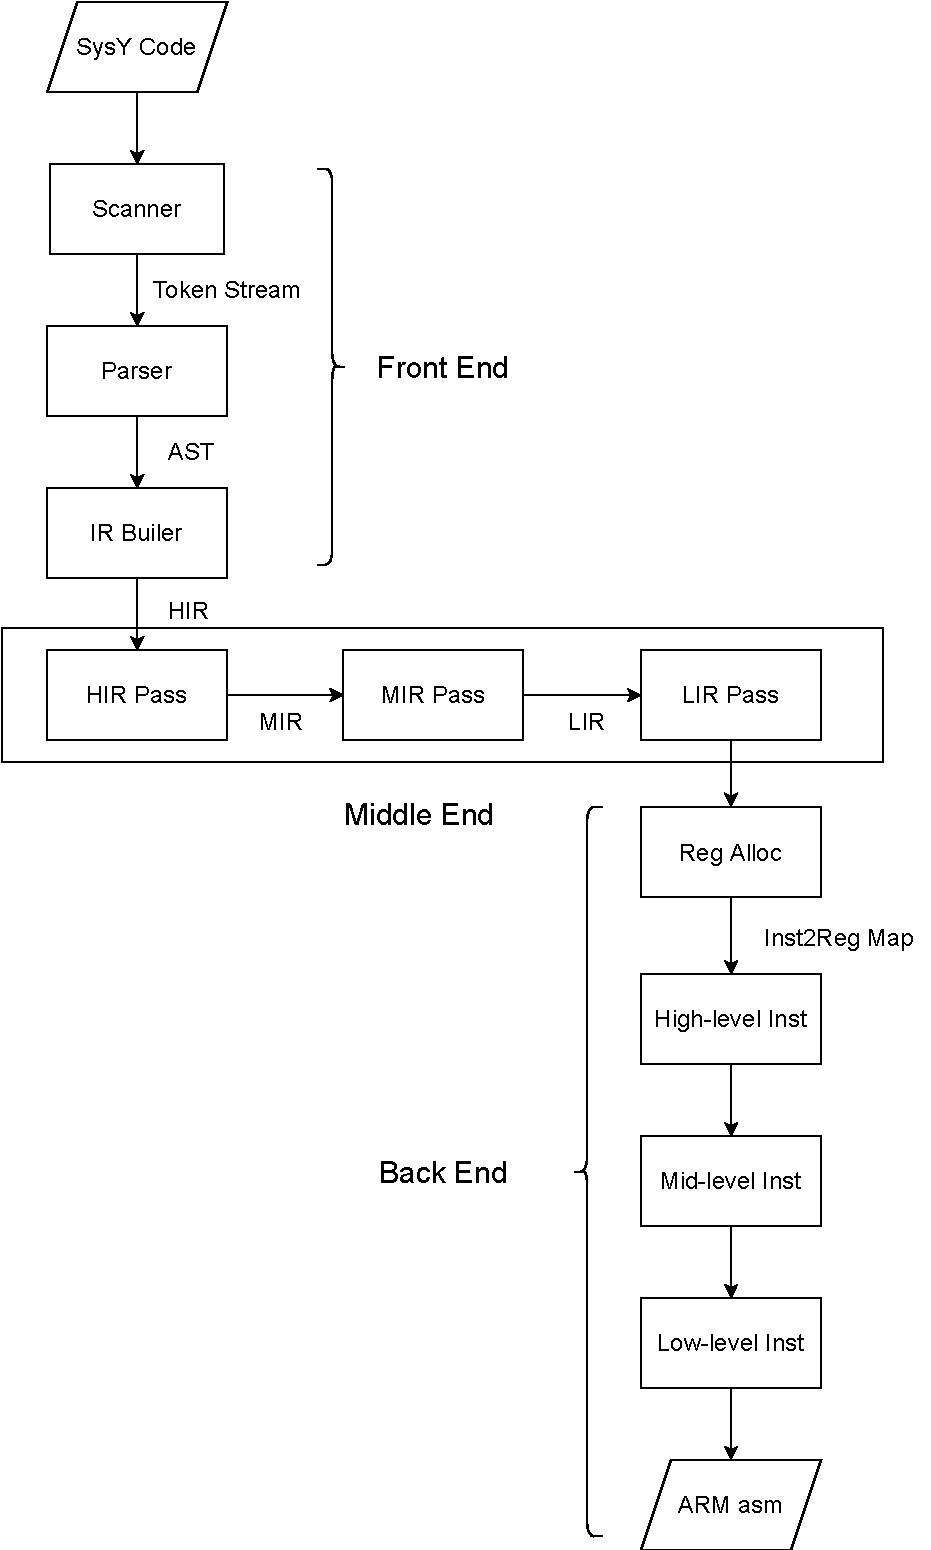
\includegraphics[width=0.8\textwidth]{figures/flammingmycompiler.pdf}
  \caption{本项目的执行流程示意图}
  \label{fig:compiler}
\end{figure}

\subsection{论文组织}

本文的剩余内容主要对上方列举的编译器中端的IR Pass中挑选几个具有代表意义的优化进行着重的理论说明和举例分析,同时兼顾后端中重要的组成部分寄存器分配算法。

第二章将介绍前端产生的IR组织方式,简要介绍由解析器生成的AST形式如何,怎样转换到中间表示,及中间表示的三层组织,并会对HIR的结构作一个简要介绍,将其与AST进行对比来说明HIR为从AST到真正IR所做的铺垫。第三章将介绍中端IR的Pass概念,即对如何对IR做优化,并举了简化控制流程图的例子来具体说明。第四章会介绍本项目中用到的IR的重要表示形式:静态单赋值形式及其构造,会介绍图论中的重要概念——支配理论。第五章介绍基于循环的优化,并举例说明之前构造的SSA对优化的设计有什么好处和简化。第六章介绍后端部分,主要是一些指令的底层化和寄存器分配算法。最后一章是对全文的总结。